% Written by Daina Chiba (daina.chiba@gmail.com).
% It was mostly copied from two poster style files:
% beamerthemeI6pd2.sty written by
%	 	Philippe Dreuw <dreuw@cs.rwth-aachen.de> and
% 		Thomas Deselaers <deselaers@cs.rwth-aachen.de>
% and beamerthemeconfposter.sty written by
%     Nathaniel Johnston (nathaniel@nathanieljohnston.com)
%		http://www.nathanieljohnston.com/2009/08/latex-poster-template/
% ---------------------------------------------------------------------------------------------------%
% Preamble
% ---------------------------------------------------------------------------------------------------%
\documentclass[final]{beamer}
\usepackage[orientation=landscape,size=custom,width=110,height=86,scale=1.2,debug]{beamerposter}
\mode<presentation>{\usetheme{RicePoster}}
\usepackage[english]{babel}
\usepackage[latin1]{inputenc}
\usepackage[T1]{fontenc}
\usepackage{amsmath,amsthm, amssymb, latexsym}

\usepackage{array,booktabs,tabularx}
\newcolumntype{Z}{>{\centering\arraybackslash}X} % centered tabularx columns


%   Begin Additional Packages
\usepackage{blindtext}
\usepackage{graphicx}
\usepackage{tikz}
%   End Additional Packages


% comment
\newcommand{\comment}[1]{}

\newlength{\columnheight}
\setlength{\columnheight}{80cm}
\newlength{\sepwid}
\newlength{\onecolwid}
\newlength{\twocolwid}
\newlength{\threecolwid}
\newlength{\restofpage}
\setlength{\sepwid}{0.024\paperwidth}
\setlength{\onecolwid}{0.24\paperwidth}
\setlength{\twocolwid}{0.4\paperwidth}
\setlength{\threecolwid}{0.19\paperwidth}
\setlength{\restofpage}{0.7\paperwidth}

% ---------------------------------------------------------------------------------------------------%
% Title, author, date, etc.
% ---------------------------------------------------------------------------------------------------%
\title{\huge deton8: Detector of Nuclei}
\author{Will LeVine \& Gabriel Vacaliuc}
\institute[Rice University]{Department of Computer Science, Rice University}
\date[Apr.2018]{April, 2018}
\def\conference{COMP540 Term Project: 2018 Data Science Bowl}
\def\yourEmail{wvl1@rice.edu,gv8@rice.edu}


% ---------------------------------------------------------------------------------------------------%
% Contents
% ---------------------------------------------------------------------------------------------------%
\begin{document}
\begin{frame}[t]

\begin{columns}[t]

\begin{column}{\onecolwid}

    \begin{block}{Introduction}
    \end{block}

    \vskip3ex

    \begin{block}{Preprocessing \& Data Whitening}
        \begin{columns}[c]
            \column{.49\textwidth}
            \begin{itemize}
                \item since the input data is of a range of sizes, we reshape all
                    images to (256, 256)
                \item we negate all images with a white background so we can 
                    assosciate brightness with nuclei
                \item since the color channels are highly correlated, we whiten
                    the data, resulting in greyscale images with reduced
                    modality effects
            \end{itemize}

            \column{.02\textwidth}

            \column{.49\textwidth}

            \begin{figure}
                \centering
                \caption{3D Plot of a sample of the training set.}
                \label{fig:correlated-features}
                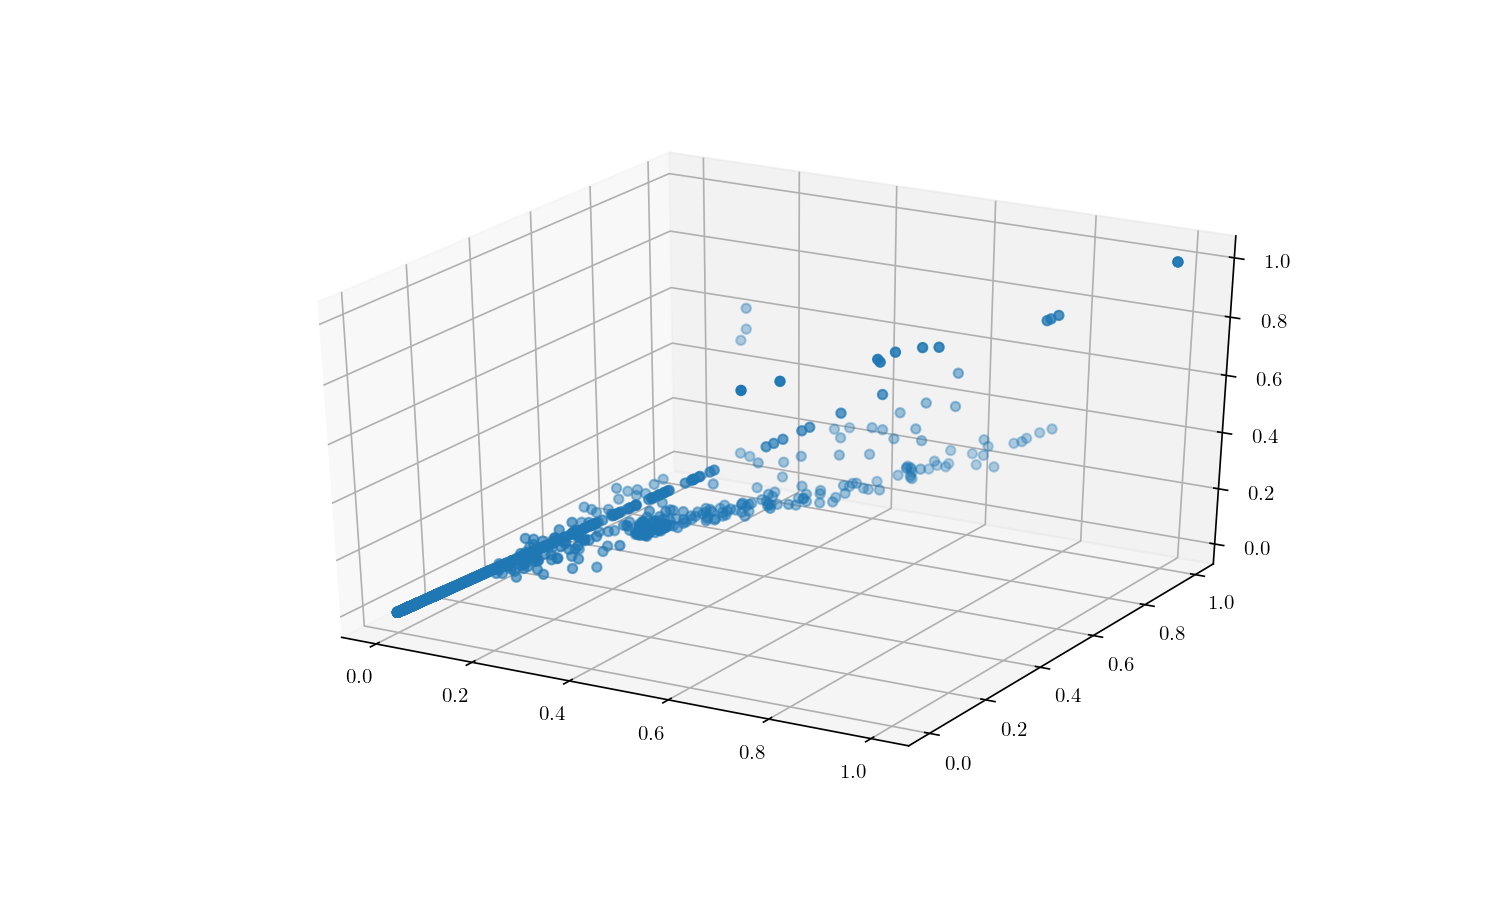
\includegraphics[width=\textwidth]{../paper/figs/correlated-features.png}
            \end{figure}
        \end{columns}

        \begin{figure}
            \centering
            \caption{Original Data.}
            \label{fig:correlated-features}
            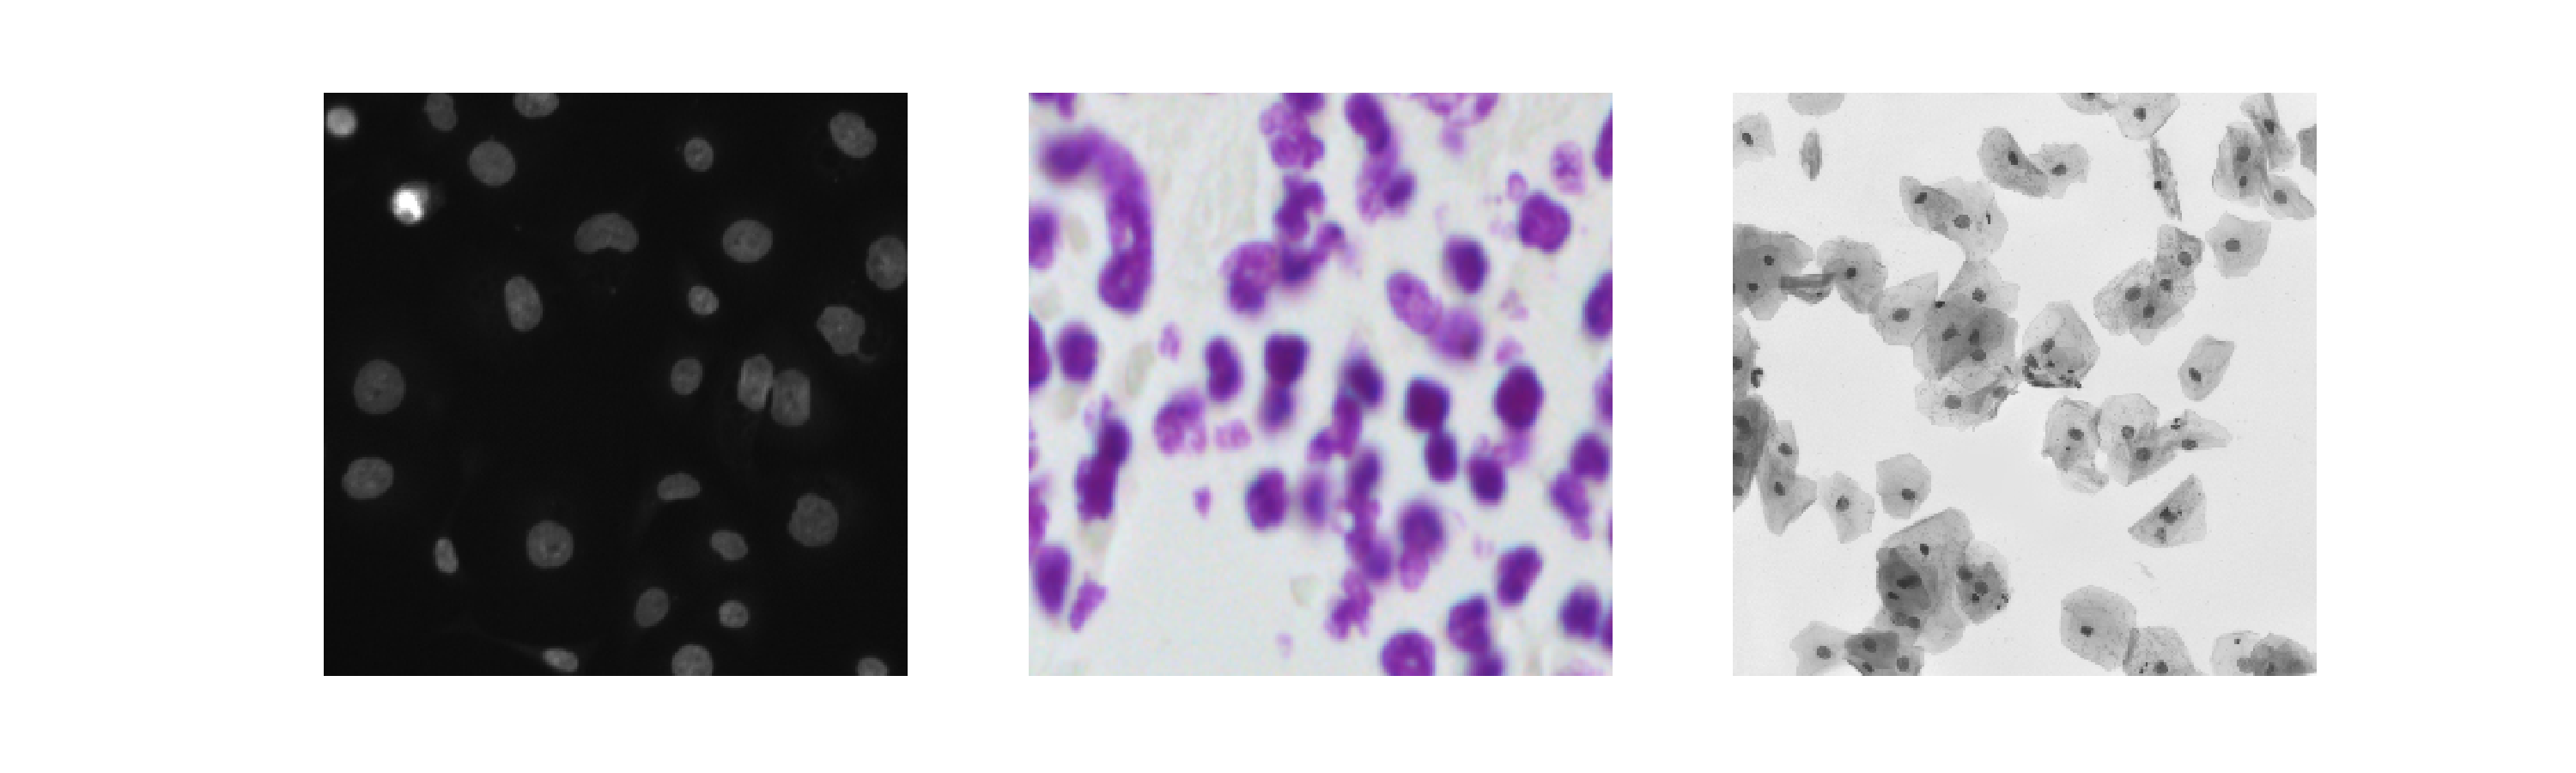
\includegraphics[width=\textwidth]{./figs/dsbowl18-imagegrid-1x3.png}
        \end{figure}

        \begin{figure}
            \centering
            \caption{Inverted and Whitened Data.}
            \label{fig:correlated-features}
            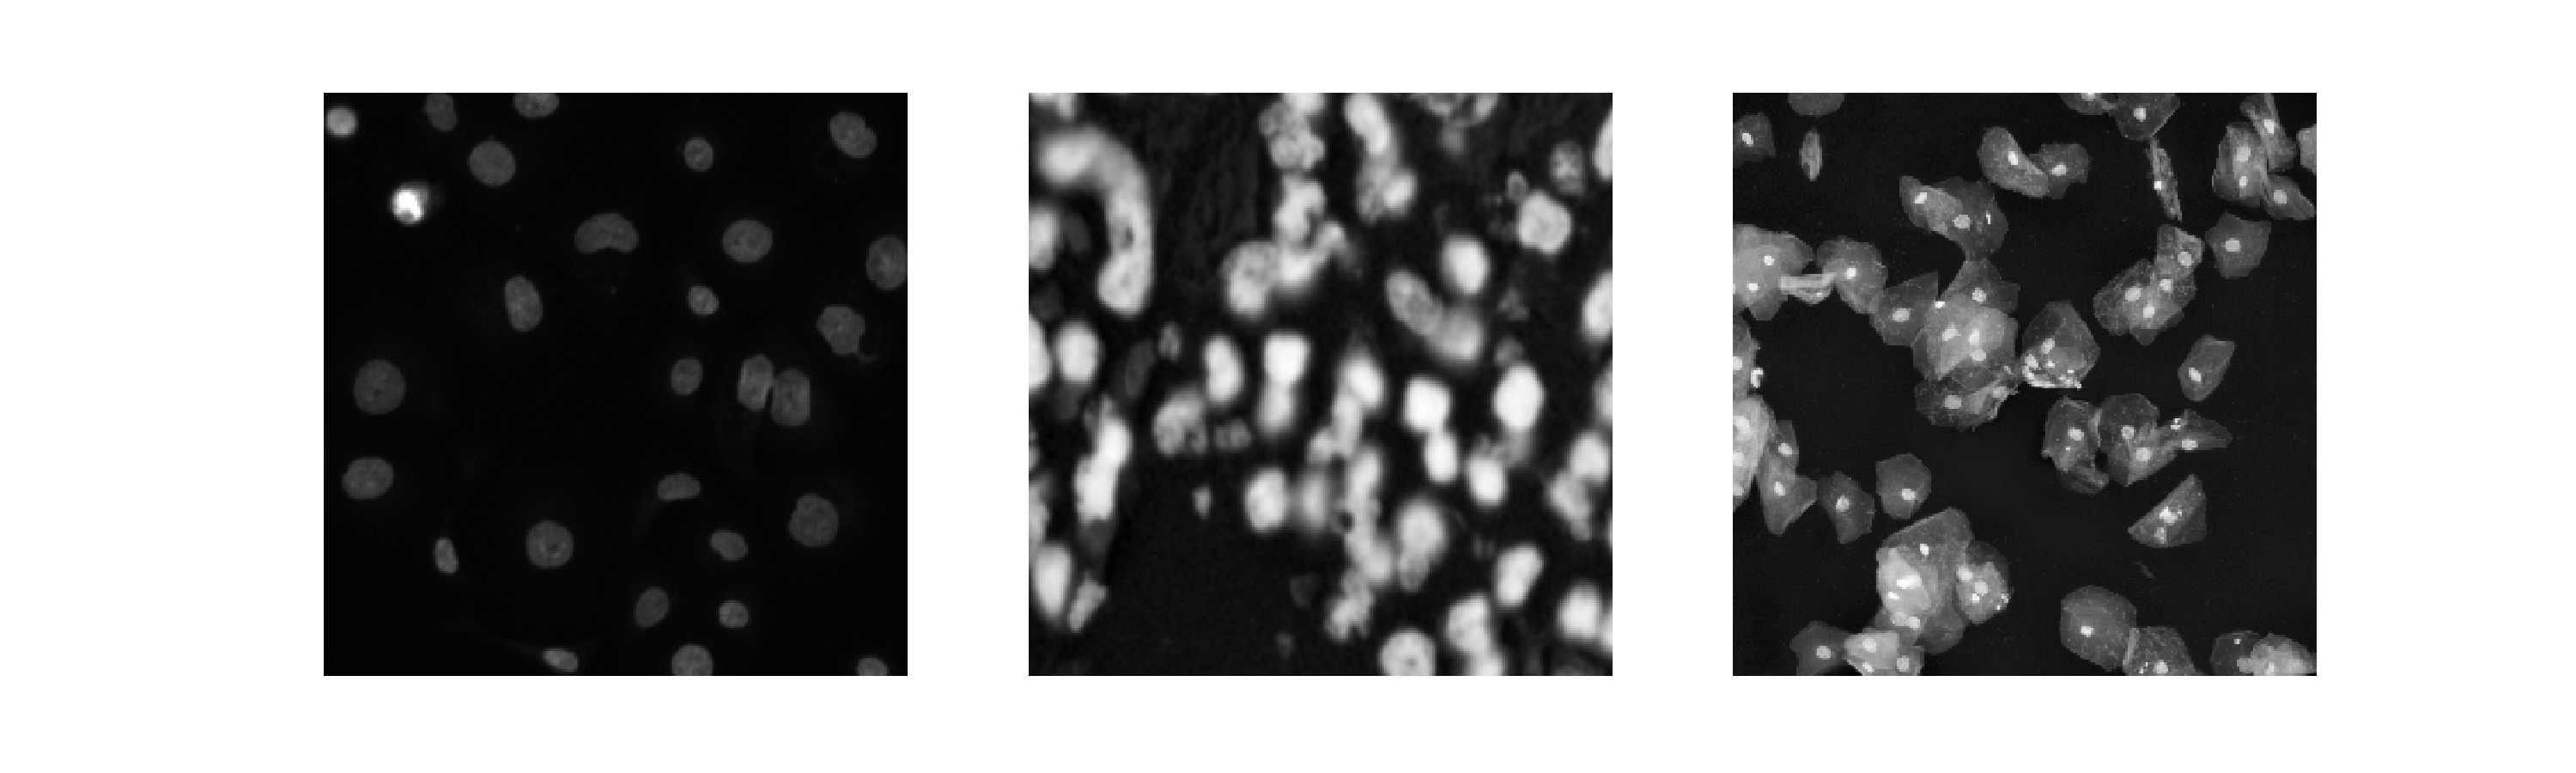
\includegraphics[width=\textwidth]{./figs/dsbowl18-imagegrid-1x3-whitened.png}
        \end{figure}

    \end{block}

    \vskip3ex

    \begin{block}{Hand Designed Features}
      \begin{itemize}
        \item Bilateral Filter: convolves image with weighted Gaussian kernel;
            denoises the image, while still preserving the edges
        \item 50/99 Image Rescaling: stretches pixel distribution; increases
            contrast between foreground and background
        \item Contrast Limited Adaptive Histogram Equalization: increases
            contrast locally; increases brightness of small nuclei
        \item Dilation: convolves image with uniform kernel; increases area of
            small nuclei
      \end{itemize}
    \end{block}

\end{column}

% -----------------------------------------------------------
% Start the second column
% -----------------------------------------------------------
\begin{column}{\restofpage}

    \begin{block}{Pipeline}
        \begin{tikzpicture}
        \node[inner sep=0pt] (raw) at (0,-12)
            {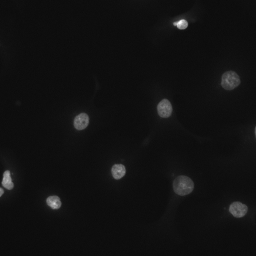
\includegraphics[width=8cm]{./figs/raw.png}};

        \node[inner sep=0pt] (bilateral) at (12,0)
            {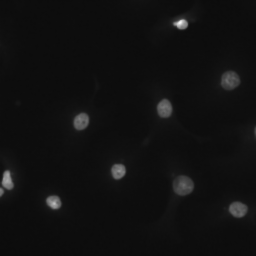
\includegraphics[width=8cm]{./figs/bilateral.png}};
        \node[inner sep=0pt] (bilateral text) at (12,-4)
            {Bilateral Filtering};
        \draw[->,line width=4pt] (raw.east) -- (bilateral.west);
        \node[inner sep=0pt] (rescale) at (12,-9)
            {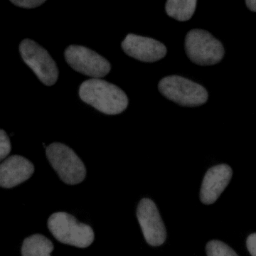
\includegraphics[width=8cm]{./figs/rescale.png}};
        \draw[->,line width=4pt] (raw.east) -- (rescale.west);
        \node[inner sep=0pt] (clahe) at (12,-18)
            {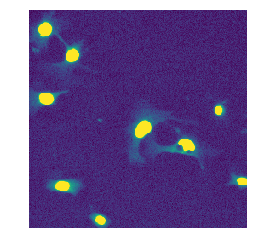
\includegraphics[width=8cm]{./figs/clahe.png}};
        \draw[->,line width=4pt] (raw.east) -- (clahe.west);
        \node[inner sep=0pt] (dilation) at (12,-27)
            {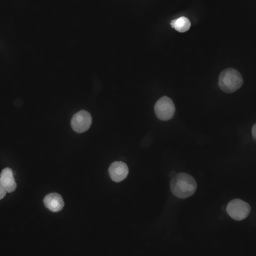
\includegraphics[width=8cm]{./figs/dilation.png}};
        \draw[->,line width=4pt] (raw.east) -- (dilation.west);

        \node[inner sep=0pt] (sgd) at (24,-9)
            {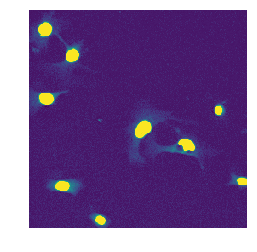
\includegraphics[width=8cm]{./figs/sgd.png}};
        \draw[-,line width=4pt] (rescale.east) -- (sgd.west);
        \draw[-,line width=4pt] (bilateral.east) -- (sgd.west);
        \draw[-,line width=4pt] (clahe.east) -- (sgd.west);
        \draw[-,line width=4pt] (dilation.east) -- (sgd.west);
        \node[inner sep=0pt] (pa) at (24,-18)
            {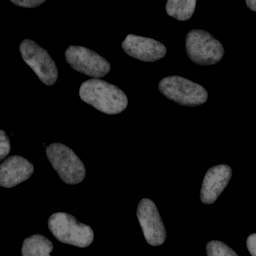
\includegraphics[width=8cm]{./figs/pa.png}};
        \draw[-,line width=4pt] (bilateral.east) -- (pa.west);
        \draw[-,line width=4pt] (rescale.east) -- (pa.west);
        \draw[-,line width=4pt] (clahe.east) -- (pa.west);
        \draw[-,line width=4pt] (dilation.east) -- (pa.west);

		\draw[fill=black,opacity=0.2,draw=black] (2.75,1.25) -- (3.75,1.25) -- (3.75,2.25) -- (2.75,2.25) -- (2.75,1.25);
		\draw[fill=black,opacity=0.2,draw=black] (2.5,1) -- (3.5,1) -- (3.5,2) -- (2.5,2) -- (2.5,1);
		\draw[fill=black,opacity=0.2,draw=black] (2.25,0.75) -- (3.25,0.75) -- (3.25,1.75) -- (2.25,1.75) -- (2.25,0.75);
		\draw[fill=black,opacity=0.2,draw=black] (2,0.5) -- (3,0.5) -- (3,1.5) -- (2,1.5) -- (2,0.5);
		\draw[fill=black,opacity=0.2,draw=black] (1.75,0.25) -- (2.75,0.25) -- (2.75,1.25) -- (1.75,1.25) -- (1.75,0.25);
		\draw[fill=black,opacity=0.2,draw=black] (1.5,0) -- (2.5,0) -- (2.5,1) -- (1.5,1) -- (1.5,0);

        \end{tikzpicture}
    \end{block}

    \begin{columns}[c]

        \column{0.33\textwidth}
        \begin{block}{a} hi \end{block}
        \column{0.33\textwidth}
        \begin{block}{b} hi \end{block}
        \column{0.33\textwidth}
        \begin{block}{c} hi \end{block}

    \end{columns}

\end{column}

\end{columns}

\end{frame}
\end{document}
